\section{Композиции алгоритмов. Градиентный бустинг}

При решении сложных задач классификации, регрессии, прогнозирования часто оказывается, что ни один из алгоритмов не обеспечивает желаемого качества восстановления зависимости. В таких случаях имеет смысл строить композиции алгоритмов, в которых ошибки отдельных алгоритмов взаимно компенсируются. Наиболее известные примеры композиций — простое и взвешенное голосование. 

\subsection{Математическая постановка задачи}

Пусть меется выборка $(x_i,y_i) , x \in R^n , y \in Y{0,1,...,K}$. Имеется задача классификации для $K$ классов. Сами классификаторы ищутся в виде

\begin{equation}
 f_k(x)=f_{k-1}(x)+\beta T(x,y)
\end{equation}
\par
 где $T(x,y)$ слабый классификатор. Т.к. имеется $K$ классов, то в итоге получится вектор из $K$ классификаторов, каждый из которых построен на основе вектора слабых классификаторов. Для классификации объектов используется метод взвешанного голосования $a(x)=\frac{1}{K}\sum_{i \in K}f_i(x)$. 

\subsection{Алгоритмы классификации}

Задача классификации — формализованная задача, в которой имеется множество объектов (ситуаций), разделённых некоторым образом на классы. Задано конечное множество объектов, для которых известно, к каким классам они относятся. Это множество называется выборкой. Классовая принадлежность остальных объектов не известна. Требуется построить алгоритм, способный классифицировать произвольный объект из исходного множества.

Классифицировать объект — значит, указать номер класса, к которому относится данный объект.

В математической статистике задачи классификации называются также задачами дискриминантного анализа. В машинном обучении задача классификации решается, как правило, с помощью методов искусственных нейронных сетей при постановке эксперимента в виде обучения с учителем.

Существуют также другие способы постановки эксперимента — обучение без учителя, но они используются для решения другой задачи — кластеризации или таксономии. В этих задачах разделение объектов обучающей выборки на классы не задаётся, и требуется классифицировать объекты только на основе их сходства друг с другом. В некоторых прикладных областях, и даже в самой математической статистике, из-за близости задач часто не различают задачи кластеризации от задач классификации.

Варианты основных алгоритмов классификации различают по количеству шагов (этапов) принятия решения, а также по степени и характеру учета статистики признаков. Так, различают одношаговые и многошаговые (последовательные) алгоритмы принятия решений. В первом варианте принятие решений предусматривает обязательную выдачу оценки $i$ номера класса $C_i$, которому принадлежит объект (с приемлемой достоверностью). Если достоверность решения невысока, то целесообразно отказаться от выбора решения на первом шаге, осуществить дополнительный набор признаков и лишь затем принять окончательное решение (или не принять и продолжить процесс наблюдения). Это так называемая последовательная стратегия принятия решения, восходящая к Вальду и его теории последовательного анализа. 

\begin{figure}
  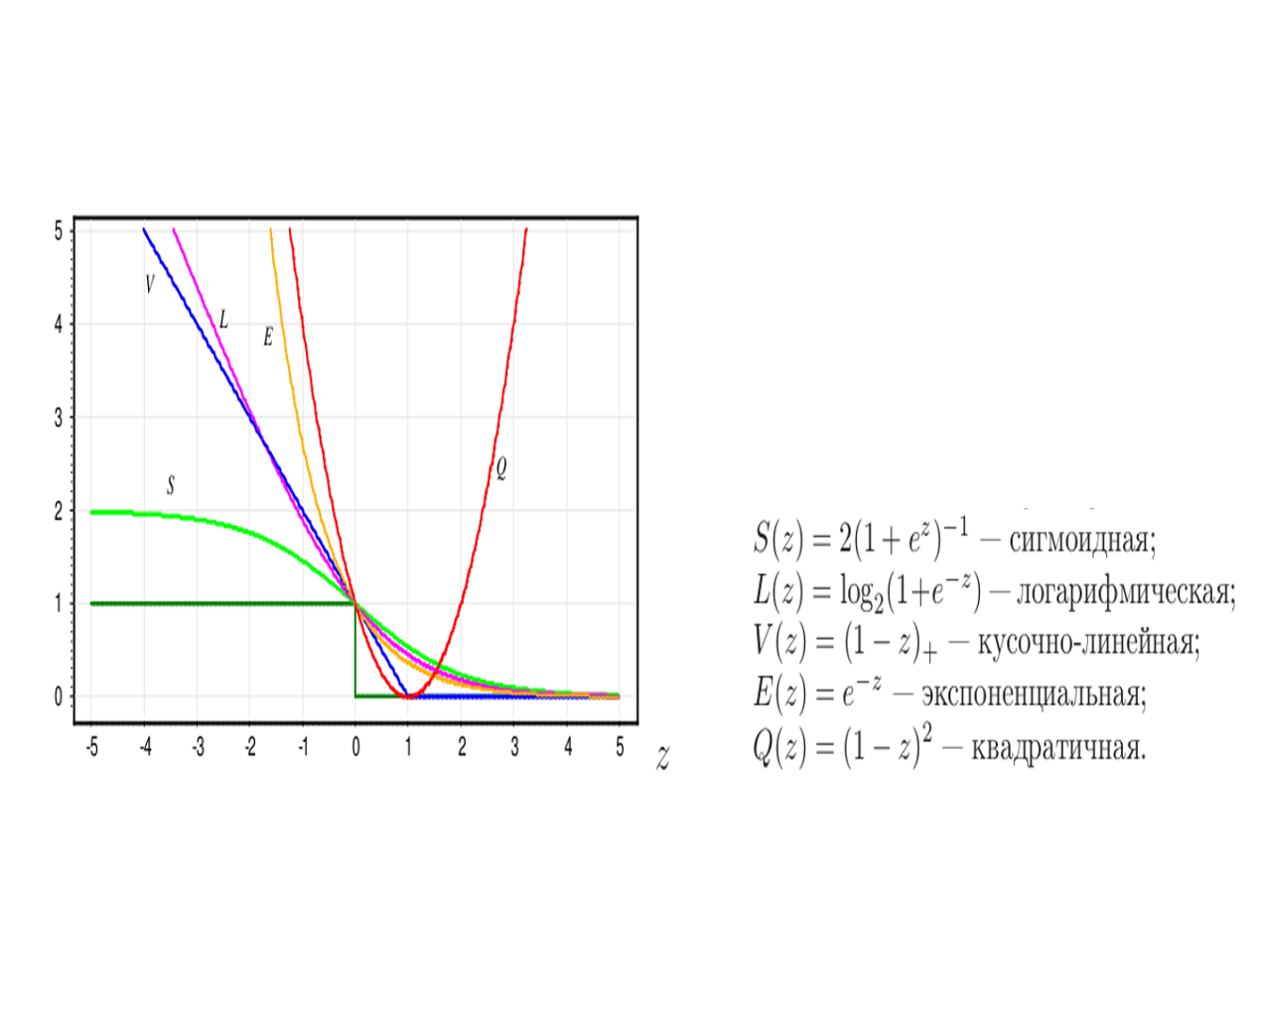
\includegraphics[height=100mm,width=\textwidth]{images/upper_approximations.png}
  \caption{Верхние пороговые аппроксимации функции потерь$|z<0|$\label{upper-approximations}}
\end{figure}

По степени учета статистических закономерностей различают синтаксические и собственно статистические алгоритмы. Из статистических алгоритмов, в свою очередь, выделяют параметрические (байесовские и небайесовские), непараметрические и нейрокомпьютерные алгоритмы. Синтаксические алгоритмы вводимые признаки учитывают качественно, часто двоичными цифрами $(0,1)$  или символами некоторого заданного алфавита. Описание признаков на языке алгебры логики - лингвистическое (кодовое, синтаксическое) служит при этом основой алгоритмов кодирования и распознавания структуры уникальных объектов. 

Параметрические байесовские алгоритмы, в отличие от небайесовских учитывают не только статистику распределений значений признаков в классах, но и определенные гипотезы об априорных вероятностях $P_i$ принадлежности объектов классам. Вероятностную структуру (статистика распределения признаков) объектов распознавания устанавливается путем предварительного натурного эксперимента, математического или физического моделирования. Введение этой информации можно трактовать как обучение распознаванию, или как адаптацию к конкретным условиям распознавания. 

Непараметрические алгоритмы синтезируют эвристически в расчете на неизвестные заранее статистические распределения признаков объектов различных классов. Они используют локальную оценку вероятности появления реализации объекта в заданной области по эмпирической частоте (на основе обучающей выборки). Это алгоритмы типа «обобщенной гистограммы» (методы парзеновского окна, ближайших соседей), алгоритмы вычисления оценок, алгебраические алгоритмы и т.д.

\subsection{Композиция алгоритмов}
Введем множество объектов $X$ и множество ответо $Y$. Наряду с этими множествами, введем вспомогательное множество $R$, называемое пространством оценок. Рассматриваются алгоритмы, имеющие вид суперпозиции $a(x)=C(b(x))$, где функция $b: X \to R$ называется алгоритмическим оператором, функция $C: R \to Y$ - решающее правило. 

Многие алгоритмы классификации имеют именно такую структуру: сначала вычисляются оценки принадлежности объекта классам, затем решающее правило переводит эти оценки в номер класса. Значением оценки $b(x)$ может быть вероятность принадлежности объекта x классу, расстояние от объекта до разделяющей поверхности, степень уверенности классификации и т.п.

Введем полное определение классификатора, на основе модели композиции. Композицией $T$ алгоритмов $a_t(x)= C(b_t(x)), t=1,\dotsc,T$ называется суперпозиция алгоритмических операторов $b_t: X \to R$, корректирующей операции  $F: R^T \to R$ и решающего правила $C: R \to Y$:


\begin{equation}
	a(x) = C(F(b_1(x),\dotsc,b_T(x))), x \in X
\end{equation}

Алгоритмы $a_t$, а иногда и операторы $b_t$ , называют базовыми алгоритмами. 
Суперпозиции вида $F(b_1,\dotsc, b_T)$ являются отображениями из $X$ в $R$, то есть, опять-таки, алгоритмическими операторами. 

Пространство оценок $R$ вводится для того, чтобы расширить множество допустимых корректирующих операций. Можно было бы определить корректирующую операцию и как отображение $F: Y^T \to Y$ , то есть комбинировать непосредственно ответы базовых алгоритмов. Однако в задачах классификации, когда множество $Y$ конечно, число «разумных» корректирующих операций такого вида невелико, что ограничивает возможность оптимизации $F$ под конкретную задачу \todobiography. Если же ком бинировать ответы алгоритмических операторов, то операция $F$ получает на входе оценки принадлежности объекта классам — более точную информацию, не огрублённую решающим правилом.

\subsection{Взвешанное голосование}

Корректирующая операция $F$ может иметь параметры, настраиваемые по обучающей выборке, наряду с параметрами базовых алгоритмов. Например, в линейной комбинации настраиваются веса $at$ базовых алгоритмов:

\begin{equation}
	b(x)=F(b_1(x), \dotsc ,b_T(x)) = \sum_{t=1}^{T} a_tb_t(x),  x \in X,  a_t \in R
\end{equation}

Если веса $a_t$ неотрицательны и нормированы, $\sum_{t=1}^{T} a_t =1$ , то композицию (1.2) называют выпуклой комбинацией базовых алгоритмов. Естественно предполагать, что вес $a_t$ тем больше, чем выше качество базового алгоритма $b_t$.

\subsection{Бустинг}

Построение бустинга лучше всего рассматривать на задаче для двух классов ${-1,1}$, а потом обобщить на общий случай, для множества классов $M$. Пусть есть двух классовая задача $Y={-1,+1}$. Допустим, что решающее правило фиксировано, $C(b) = sign(b)$, базовые алгоритмы возвращают ответы $-1,0,+1$. Ответ $b_t(x) = 0$ означает, что базовый алгоритм $b_t$ отказывается от классификации объекта $x$, и ответ $b_t(x)$ не учитывается в композиции.
Искомая алгоритмическая композиция имеет вид:
\begin{equation}
	a(x)=C(F(b_1(x),\dotsc,b_T(x)))=sign(\sum_{t=1}^{T} a_tb_t(x)), x \in X
\end{equation}

Определим функционал качества композиции как число ошибок, допускаемых
ею на обучающей выборке:
\begin{equation}
	Q_T=\sum_{t=1}^{l} y_i\sum_{t=1}^{T} a_tb_t < 0]
\end{equation}

Напрямую, оптимизировать такой функционал очень сложно, поэтому заменим его на оценку сверху:
\begin{equation}
	Q_T=min_{\beta_m,\gamma_m}\sum_{i=1}^{N}L(y_i,\sum_{m=1}^{M}\beta_m b(x_i;\gamma_m)))
\end{equation}
В качестве функции потерь $L(y_i,f_m(x;\gamma)$ могут выступать функции, приведенные на ~\ref{upper-approximations}.
Общий алгоритм бустинга:

\begin{algorithm}
  \caption{Общий алгоритм бустинга}
  \label{overall-boosting-algorithm}
  \begin{enumerate}
  \item Инициализировать переменные $f_0(x)=0$
  \item Для каждого шага $m=1,2 .. M$:
    \begin{enumerate}
      \item Вычисляем $(\beta_m,\gamma_m)=arg \min_{\beta,\gamma} \sum_{i=1}^{N}L(y_i,f_{m-1}(x_i)+\beta b(x_i;\gamma))$
      \item $f_m(x)=f_{m-1}(x)+\beta_m b(x;\gamma_m)$
    \end{enumerate}
  \end{enumerate}
\end{algorithm}


\subsection{Градиентный бустинг}

Пусть дана обучающая выборка ${x_i,y_i}, i=1,..,N, y \in K$. Будем строить классификаторы, имеющие вид $f_k(x_i)=f_k(x_{i-1})+\gamma_i b_k(x_i)$ где $b(x_i) $ классификатор. В конечном итоге у нас будет $k$ классификаторов вида $f_k(x_i), k=1,...,K$ и классификация будет происходить по голосованию большинства. Для этой задачи введем экспоненциальную функцию потерь $e^{f(x_i,y_i)}$. Для множества классов $K$ данная функция имеет вид:
\begin{equation}
  p(x_ik)= \frac{e^{f_k(x_i)}}{\sum_{l=1}^{K}f_l(x_i)}
\end{equation}

В качестве слабых классификаторов будем использовать решающие деревья. По  решающее дерево можно представить в виде набора правил, или конъюнкций вида $T(x) = \sum_{i=1}^{J}R_i[x \in R_i]$, где $[x \in R_i]$ - по нотации хайденгера обозначает $0$ если условие $[x \in R_i]$ ложно, иначе $1$.

С учетом этих предположений, алгоритм градиентного бустинга приведен в алгоритме 2.


\begin{algorithm}
  \caption{Градиентный бустинг для многоклассовой классификации}
  \label{gradient-boosting-algorithm}
  \begin{enumerate}
  \item Инициализировать переменные $f_0(x)=0, k=1,2,...,K$
  \item Для каждого шага $m=1,2 .. M$:
    \begin{enumerate}
      \item Вычислить:
      \begin{equation}
      	p_k(x)=\frac{e^{f_k(x)}}{\sum_{l=1}^{K}e^{f_l(x)}}, k=1,2,...,K
      \end{equation}
      \item Для k = 1 до K:
      \begin{enumerate}
      	\item $r_{ikm}=y_{ik}-p_k(x_i), i=1,2,...,N$, где $y_{ik}=1$ если $y_i$ принадлежит классу $k$, иначе 0.
      	\item Для множества пар $(x_i,r_ikm)$ построить решающее дерево. С конечными регионами: $R_{jkm}, j=1,2,...,J_m$
      	\item $\gamma_{jkm}=\frac{K-1}{K}\frac{\sum_{x_i\in R_{jkm}}r_{ikm}}{\sum_{x_i\in R_{jkm}}|r_{ikm}|(1-|r_{ikm}|})$
      	\item Обновить $f_{km}=f_{k,m-1}(x)+\sum_{j=1}^{J_m}\gamma_{jkm}I(x\in R_{jkm}$
      \end{enumerate}
    \end{enumerate}
    \item Выход: $f_k=f_{km}(x), k=1,2,...,K$
  \end{enumerate}
\end{algorithm}

\subsection{Заключение}


Преимущества бустинга.


На сегодняшний день является одним из самых мощных алгоритмов распознавания и машинного обучения. Это достигается благодаря вышеупомянутой адаптивной технике построения композиции. К тому же, бустинг предоставляет множество возможностей для вариаций. 

\begin{itemize}
    \item Можно рассматривать различные функции потерь. Это позволяет решать как задачи классификации, так и задачи регрессии. К тому же, возможность выбора произвольной функции потерь позволяет акцентировать внимание на особенностях данных в задаче.

    \item Возможно рассмотрение любого семейства базовых алгоритмов. А это, опять же, дает широкиие возможности учета особенностей даннной задачи. Бустинг над решающими деревьями считается одним из наиболее эффективных вариантов бустинга. А учитывая, что решающие деревья в свою очередь тоже используют базовые алгоритмы (например, пороговые, линейные и т.п.), в результате получается огромное количество вариантов для настройки.

    \item Благодаря достаточной простоте метода и четкому математическому обоснованию, в каждой конкретной вариации бустинга не сложно провести некоторые математические и алгоритмические оптимизации, которые заметно ускорят работу алгоритма.
\end{itemize}

Недостатки бустинга

\begin{itemize}

\item Бустинг – трудоемкий метод, и работает он достаточно медленно. Зачастую требуется построение сотен или даже тысяч базовых алгоритмов для композиции. 

\item Без дополнительных модификаций он имеет свойство полностью подстраиваться под данные, в том числе под ошибки и выбросы в них.

\item Идея бустинга обычно плохо применима к построению композиции из достаточно сложных и мощных алгоритмов. Построение такой композиции занимает очень много времени, а качество существенно не увеличивается. В-четвертых, результаты работы бустинга сложно интерпретируемы, особенно если в композицию входят десятки алгоритмов.

\end{itemize}

\newpage